\chapter{Solvers for SDEs}
We now consider the stochastic differential equation (SDE) on the form

\begin{align}
    dx(t) &= f(t,x(t),p_f)dt + g(t,x(t),p_g)d\omega(t) \\
    d\omega & \sim N_{iid}(0,I dt)
\end{align}

where $x\in \probR^{n_x}$ and $\omega$ is Brownian motion with dimension $n_\omega$. $p_f$ and $p_g$ are parameters for the drift and the diffusion term respectively. 

\section{Multivariate Wiener process}
Before we can start simulating any SDEs, we need to have a way of generating realizations of Brownian motion. Brownian motion is defined as the integral of \textit{random noise}, which is a complex mathematical construction that does not exist in real life. Furthermore, Brownian motion is a fractal, meaning that its behaviour is scale indifferent, i.e., if you "zoom in" the pattern repeats itself indefinitely. Brownian motion is defined as a continuous function with mean $0$, and variance $t$. Brownian motion was discovered by the English botanist, Brown, as he saw pollen moving due to molecules bumping into each other. This later lead to the discovery of molecules, and precise estimation of the number of molecules in a mole. Sometimes Brownian motion is called \textit{the Wiener process}, hence we might denote it $\omega$. Listing \ref{lst4:bm} is a Matlab implementation of a function that simulates a realization of a multivariate Brownian motion. 

\begin{lstlisting}[language=Matlab,caption=Simulation of multivariate Brownian motion,label=lst4:bm]
function [W,Tw,dW] = StdWienerProcess(T,N,nW,Ns,seed)
    % StdWienerProcess Ns realizations of a standard Wiener process
    %
    % Syntax: [W,Tw,dW] = StdWienerProcess(T,N,Ns,seed)
    % W : Standard Wiener process in [0,T]
     %Tw : Time points
     %dW : White noise used to generate the Wiener process
    %
    % T : Final time
    % N : Number of intervals
    % nW : Dimension of W(k)
    % Ns : Number of realizations
    % seed : To set the random number generator (optional)
    if nargin == 4
        rng(seed);
    end
    dt = T/N;
    dW = sqrt(dt)*randn(nW,N,Ns);
    W = [zeros(nW,1,Ns) cumsum(dW,2)];
    Tw = 0:dt:T;
\end{lstlisting}

Figure \ref{fig4:2dBM} shows three realizations of 2D standard Brownian motion. 

\begin{figure}[H]
    \centering
    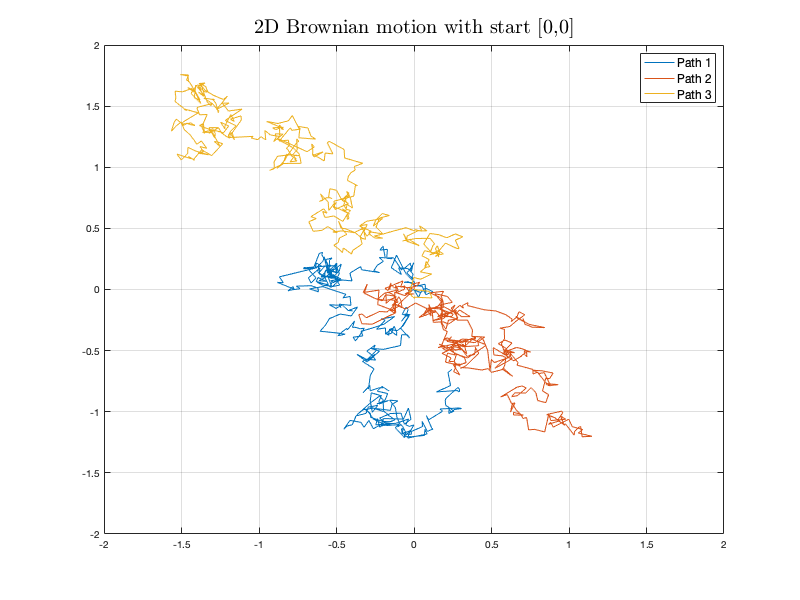
\includegraphics[width=\textwidth]{graphics/opg4/2dBM.png}
    \caption{Three realizations of 2D standard Wiener process}
    \label{fig4:2dBM}
\end{figure}



\section{Implementation of Euler-Manayam}
Given a SDE, we want to be able to simulate sample paths. To do this, we need to be able to solve the SDE numerically. Generally, speaking SDEs are often solved by the stochastic analogue to the explicit Euler method, i.e., 1. order Taylor with left-bound starting point, to solve the stochastic part. In fact, this is so pronounced that there is an entire algebra that is based on this principle known as It$\Bar{\text{o}}$ calculus, after the Japanese mathematician. 

The first approach, and perhaps most natural, is to use explicit Euler for both the drift and the diffusion term. This is known as the explicit-explicit method or alternatively \textit{Euler-Manayama}. The method is based upon

\begin{align}
    x(t+h) - x(t) &= f(t,x(t),p_f)h + g(t,x(t),p_g)(\omega(t+h)-\omega(t)) \\
    x(t+h) &= x(t) + f(t,x(t),p_f)h + g(t,x(t),p_g)(\omega(t+h)-\omega(t)).
\end{align} 

Listing \ref{lst4:EE} shows the Matlab implementation of the explicit-explicit method.


\begin{lstlisting}[language=Matlab,caption=Implementation of Euler-Manayama,label=lst4:EE]
function [x,f,J] = SDENewton(ffun,t,dt,psi,xinit,tol,maxit,varargin)
    I = eye(length(xinit));
    x = xinit;
    [f,J] = feval(ffun,t,x,varargin{:});
    R = x - f*dt - psi;
    it = 1;
    while ( (norm(R,'inf') > tol) && (it <= maxit) )
        dRdx = I - J*dt;
        mdx = dRdx\R;
        x = x - mdx;
        [f,J] = feval(ffun,t,x,varargin{:});
        R = x - f*dt - psi;
        it = it+1;
    end
\end{lstlisting}



\section{Implementation of implicit-explicit}
Another approach to solving the SDE is to combine an implicit and an explicit method. To maintain the consistency wrt ordinary stochastic calculus the diffusion term is still treated by an explicit method, however, the drift term is now solved by an implicit Euler method. Hence the method is based upon

\begin{align}
    x(t+h) - x(t) = f(t+h,x(t+h),p_f)h + g(t,x(t),p_g)(\omega(t+h)-\omega(t)) \\
    x(t+h) - x(t) - f(t+h,x(t+h),p_f)h - g(t,x(t),p_g)(\omega(t+h)-\omega(t)) = 0.
\end{align} 

The latter can be solved by using Newton method (alternatively inexact Newton). Listing \ref{lst4:IE} shows the Matlab implementation of the implicit-explicit method.

\begin{lstlisting}[language=Matlab,caption=Implementation of the implicit-explicit method for SDEs,label=lst4:IE]
function X=SDEimplicit(ffun,gfun,T,x0,W,varargin)
    tol = 1.0e-8;
    maxit = 100;

    N = length(T);
    nx = length(x0);
    X = zeros(nx,N);

    X(:,1) = x0;
    k=1;
    [f,~] = feval(ffun,T(k),X(:,k),varargin{:});

    for k=1:N-1
        g = feval(gfun,T(k),X(:,k),varargin{:});
        dt = T(k+1)-T(k);
        dW = W(:,k+1)-W(:,k);
        psi = X(:,k) + g*dW;
        xinit = psi + f*dt;
        [X(:,k+1),f,~] = SDENewton(ffun, T(:,k+1), dt, psi, xinit, tol, maxit, varargin{:});
    end
\end{lstlisting}


\section{Test on stochastic Van der Pol}
Now that we have made an implementation of the both and explicit-explicit and an implicit-explicit method with fixed step size we want to compare these. To do so we look at the Van der Pol problem given by
\begin{align}
    \Ddot{x}(t) &= \mu (1-x(t)^2) \dot{x}(t) - x(t).
\end{align}
To solve the problem using the explicit Euler method we must first re-write the problem as a system of first order differential equations. Luckily this is done easily and given by

\begin{align}
    \dot{x}_1(t) &= x_2(t) \\
    \dot{x}_2(t) &= \mu(1-x_1(t)^2) x_2(t) - x_1(t).
\end{align}

Since we are looking at SDEs, we will use a stochastic version of the system. Van der Pol with state \textit{independent} diffusion is given by

\begin{align}
    dx_1(t) &= x_2(t)dt \\
    dx_2(t) &= \left[\mu(1-x_1(t)^2) x_2(t) - x_1(t)\right] dt + \sigma d\omega (t).
\end{align}

The Van der Pol problem with state \textit{dependent} diffusion is given by

\begin{align}
    dx_1(t) &= x_2(t)dt \\
    dx_2(t) &= \left[\mu(1-x_1(t)^2) x_2(t) - x_1(t)\right] dt + \sigma\left(1+ x_1(t)^2\right) d\omega (t).
\end{align}

We will now test the explicit Euler method on the Van der Pol problem with $\mu \{3,20\}$,  $x_1(0)=x_2(0)=0.5$ and $\sigma \in \{1,2\}$, with both state dependent and state independent diffusion terms.

\subsection{Explicit-explicit}
Figure \ref{fig4:ex_indep} shows realization of solution to the stochastic Van der Pol problem with state independent diffusion solved with Euler-Manayama. From the plot it is evident that faster dynamic given when $\mu=20$ reduce the relative effect of the diffusion term. Therefore, the system with $\mu=20$ exhibit less stochastic behaviour.

It is also evident that increasing the diffusion parameter, $\sigma$, increases the stochasticity in the system. The realization with high diffusion parameter have visibly more variance. 

\begin{figure}[H]
    \centering
    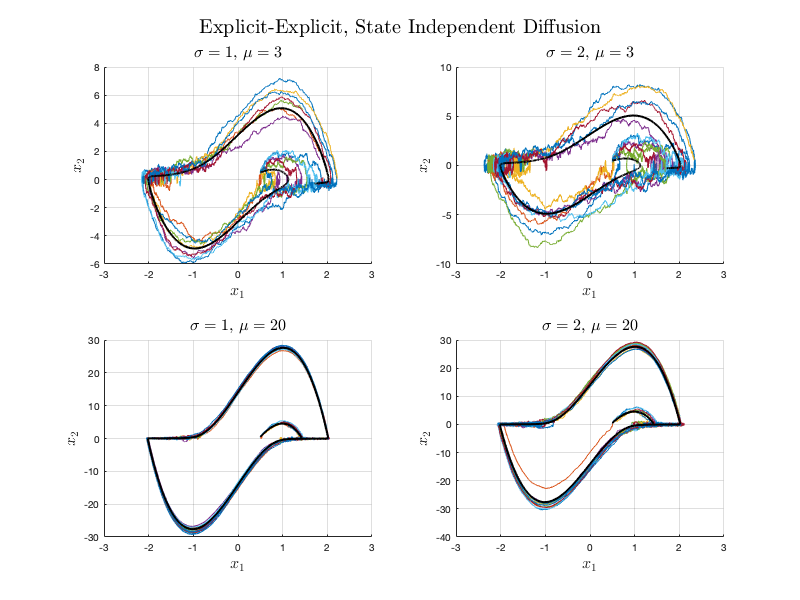
\includegraphics[width=\textwidth]{graphics/opg4/ex_indep.png}
    \caption{Explicit-explicit solution with state independent diffusion}
    \label{fig4:ex_indep}
\end{figure}


Figure \ref{fig4:ex_dep} shows realization of solution to the stochastic Van der Pol problem with state dependent diffusion again solved with Euler-Manayama. From the plot we can see quite different behaviour compared with the realizations for state independent diffusion. Specifically, the stochasticity is more pronounced when $|x_1|$ is large, i.e., in the left- and right hand side of the plots.  

This time the effect of increasing the diffusion parameter, $\sigma$, increases the stochasticity in the system even more than before. Before we mainly saw a difference in variance for the low value of $\mu$. This time we also see a big difference where $\mu=20$.

\begin{figure}[H]
    \centering
    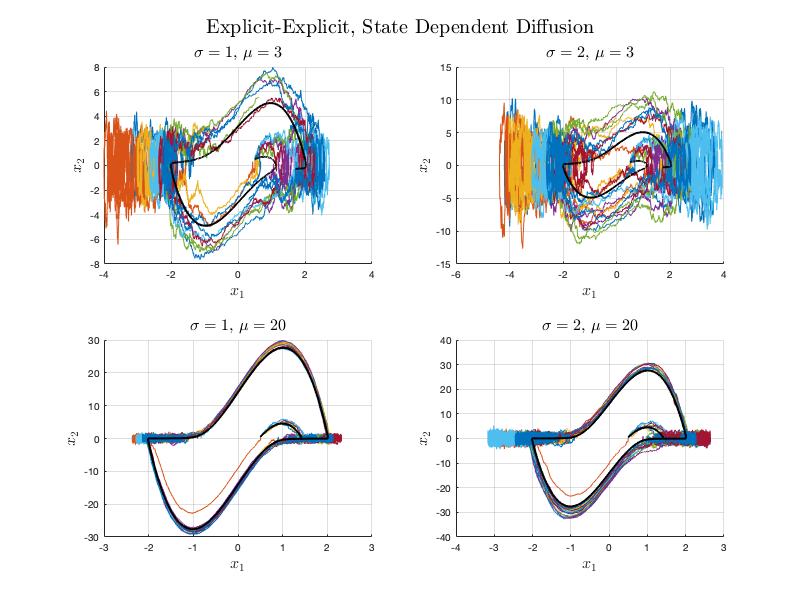
\includegraphics[width=\textwidth]{graphics/opg4/ex_dep.png}
    \caption{Explicit-explicit solution with state dependent diffusion}
    \label{fig4:ex_dep}
\end{figure}

\subsection{Implicit-explicit}
Figure \ref{fig4:im_indep} shows realization of solution to the stochastic Van der Pol problem with state independent diffusion solved with an implicit-explicit method. From the plot it is evident that faster dynamic given when $\mu=20$ reduce the relative effect of the diffusion term. Therefore, the system with $\mu=20$ exhibit less stochastic behaviour.

It is also evident that increasing the diffusion parameter, $\sigma$, increases the stochasticity in the system. The realization with high diffusion parameter have visibly more variance. 

\begin{figure}[H]
    \centering
    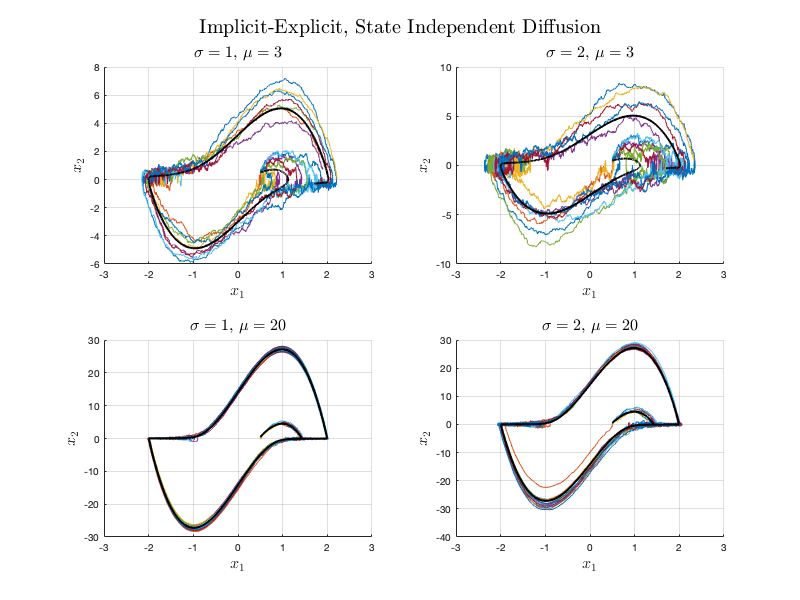
\includegraphics[width=\textwidth]{graphics/opg4/im_indep.png}
    \caption{Implicit-explicit solution with state independent diffusion}
    \label{fig4:im_indep}
\end{figure}


Figure \ref{fig4:im_dep} shows realization of solution to the stochastic Van der Pol problem with state dependent diffusion again solved with an implicit-explicit method. From the plot we can see quite different behaviour compared with the realizations for state independent diffusion. Specifically, the stochasticity is more pronounced when $|x_1|$ is large, i.e., in the left- and right hand side of the plots.  

This time the effect of increasing the diffusion parameter, $\sigma$, increases the stochasticity in the system even more than before. Before we mainly saw a difference in variance for the low value of $\mu$. This time we also see a big difference where $\mu=20$.

Overall, the difference between the solutions with the explicit-explicit and implicit-explicit method is very small. By visual inspections of the realization it is not possible to tell the solution curves apart---however, for particularly stiff systems the implicit-explicit method might not require as many function calls. 


\begin{figure}[H]
    \centering
    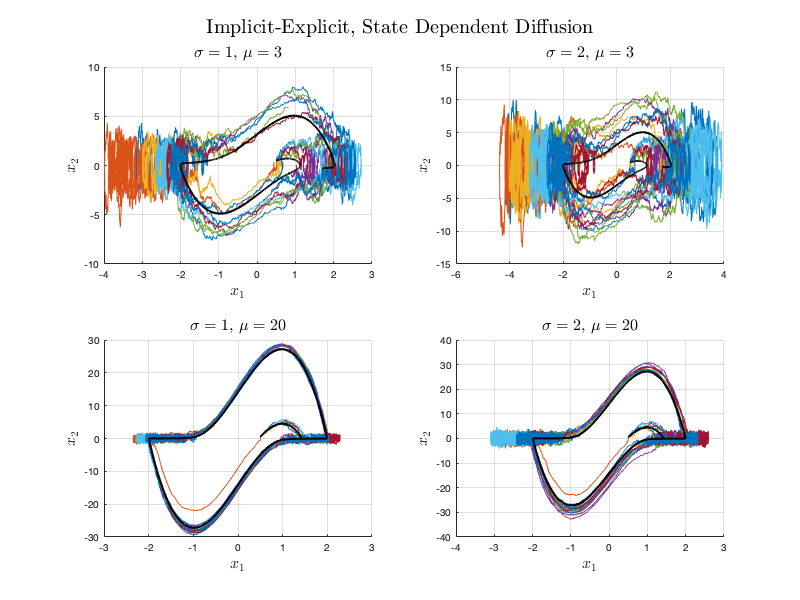
\includegraphics[width=\textwidth]{graphics/opg4/im_dep.png}
    \caption{Implicit-explicit solution with state dependent diffusion}
    \label{fig4:im_dep}
\end{figure}


\subsection{Weak vs strong convergence}
Generally, the goal of numerical methods is to approximate systems of differential equation as good as possible with as little computational cost as possible. A requirement for such numerical methods is some consistency, i.e., the approximation should become arbitrarily good when the step size becomes arbitrarily small. To this end, we have introduced the notion of \textit{order}. 

We say that a method as order $p$ whenever $e = \mathcal{O}(h^p)$, where $e$ is the errors and $h$ is the step size. Naturally, we want the order to be as big as possible (we generally use $h<1$). However, for stochastic methods it is not as simple. For stochastic systems we can measure both the accuracy of the mean, known as \textit{strong convergence}. Alternatively, we can measure the accuracy of the statistics of the individual trajectories at the end point---known as \textit{weak convergence}. 

Euler-Manayama has weak order 1, but only strong order 0.5. This means that for very noisy systems, we might require a very low step size. Figure \ref{fig4:sde_order} shows solutions to realizations to the stochastic Van der Pol together with solution to the deterministic system. Notice that for the same step size the stochastic system might diverge while the deterministic does not. This is because of the difference between the strong and weak convergence of the Euler-Manayama scheme. 

\begin{figure}[H]
    \centering
    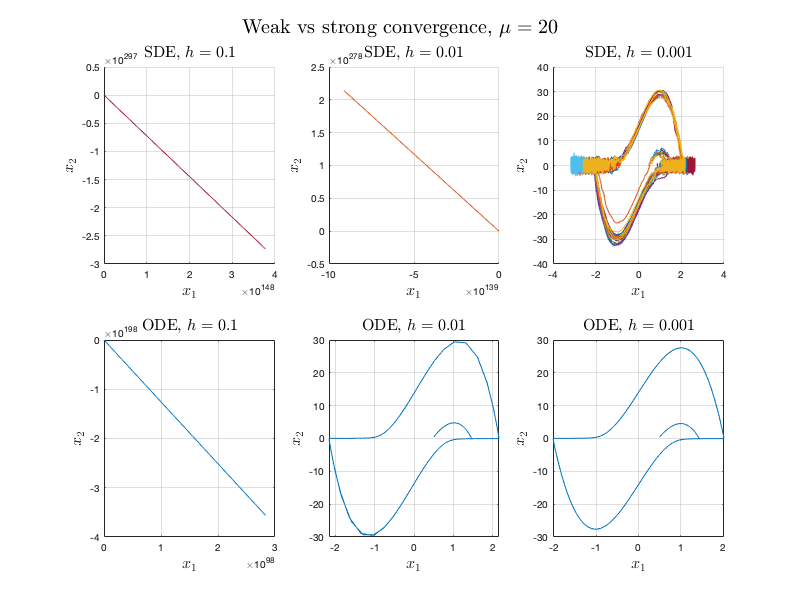
\includegraphics[width=\textwidth]{graphics/opg4/sde_order.png}
    \caption{Implicit-explicit solution with state dependent diffusion}
    \label{fig4:sde_order}
\end{figure}





